\documentclass[sigconf]{acmart}
\usepackage{booktabs}
\usepackage{algorithm}
\usepackage{algpseudocode}


%% \BibTeX command to typeset BibTeX logo in the docs
\AtBeginDocument{%
  \providecommand\BibTeX{{%
    \normalfont B\kern-0.5em{\scshape i\kern-0.25em b}\kern-0.8em\TeX}}}

%% These commands are for a PROCEEDINGS abstract or paper.
\settopmatter{printacmref=false} % Removes citation information below abstract
\renewcommand\footnotetextcopyrightpermission[1]{} % removes footnote with conference information in 

\acmConference[AEPRO 2023]{AEPRO 2023: Algorithm Engineering Projects}{March 15}{Jena, Germany}

% convert text to title case
% http://individed.com/code/to-title-case/

% that helps you to formulate your sentences
% https://www.deepl.com/translator

\begin{document}

%%
%% The "title" command has an optional parameter,
%% allowing the author to define a "short title" to be used in page headers.
\title[Generierung von visuell unterschiedlichen 2D Datensätzen mit ähnlichen statistischen Eigenschaften ]{Generierung von visuell unterschiedliche 2D Datensätzen mit ähnlichen statistischen Eigenschaften\\\large Algorithm Engineering 2023 Project Paper}

%%
%% The "author" command and its associated commands are used to define
%% the authors and their affiliations.

\author{Eric Kaufmann}
\affiliation{%
  \institution{Friedrich Schiller University Jena}
  \country{Germany}}
\email{eric.kaufmann@uni-jena.de}

\author{Benjamin Schneg}
\affiliation{%
  \institution{Friedrich Schiller University Jena}
  \country{Germany}}
\email{benjamin.schneg@uni-jena.de}

%% The abstract is a short summary of the work to be presented in the article.
\begin{abstract}

The five-finger pattern \cite{macgilchrist2014}:
\begin{enumerate}
\item \textbf{Topic and background:} What topic does the paper deal with? What is the point of departure for your research? Why are you studying this now?
\item \textbf{Focus:} What is your research question? What are you studying precisely?
\item \textbf{Method:} What did you do?
\item \textbf{Key findings:} What did you discover?
\item \textbf{Conclusions or implications:} What do these findings mean? What broader issues do they speak to?
\end{enumerate}


\end{abstract}

%%
%% Keywords. The author(s) should pick words that accurately describe
%% the work being presented. Separate the keywords with commas.
\keywords{entity resolution, data cleansing, programming contest}


%%
%% This command processes the author and affiliation and title
%% information and builds the first part of the formatted document.
\maketitle

\let\thefootnote\relax\footnotetext{AEPRO 2023, March 1, Jena, Germany. Copyright \copyright 2023 for this paper by its authors. Use permitted under Creative Commons License Attribution 4.0 International (CC BY 4.0).}


\section{Introduction}

In der Statistik ist die Analyse von Datensätzen maßgeblich. Bei besonders großen bzw. komplex strukturierten Datenmengen ist es häufig schwierig die Daten sinnvoll zu visualisieren. Demnach wird der Datensatz nur von Eigenschaften, wie dem Mittelwert oder der Standardabweichung, klassifiziert. Dabei können Datensätze, die sich visuell kaum ähnlich sind, dennoch nahezu identische statistische Eigenschaften aufweisen. 

\subsection{Background}

Um Datensätze zu generieren, die bis auf einen bestimmten Fehler, die gleichen statistischen Eigenschaften aufweist, wird der Ansatz des Simmulated Annealing verwendet. Die Idee ist dabei iterativ ein Problem näher an seine Optimallösung zu bringen. Es wird dabei akzeptiert, dass man am Anfang größere Fehler zulässt, diese Toleranz (Temperatur) jedoch über die Interationen nachlässt. Das heißt, das nach jeder Iteration die erlaubte Veränderung gedämpft wird, sodass man exakter die Lösung approximieren kann.

\subsection{Related Work}

Die Idee basiert auf auf der Veröffentlichung \textit{Same Stats, Different Graphs: Generating Datasets with Varied Appearance and Identical Statistics through Simulated Annealing} von Matejka und Fitzmaurice. Dort wurde ein zweidimensionaler Datensätze mittels Simmulated Annealing auf eine Zielstruktur transformiert. Sowohl der initiale als auch der transformierte Datensatz wiesen dabei einen ähnlichen Mittelwert, eine ähnliche Standwardabweichung und ähnlichen Korrelationskoeffizient auf. Ähnlich wurde dort mit einer Gleichheit auf von bis zu zwei Nachkommastellen definiert.

\subsection{Our Contributions}

In dieser Veröffentlichen wurde nun die Idee von Matejka und Fitzmaurice aufgegriffen und optimiert. Anstatt den neuen Datensatz mittels Python zu gegerieren, wurde in dieser Arbeit versucht durch die Verwendung von C++ und OpenMP eine effizientere Lösung zu finden.  

%\subsection{Outline}



\section{The Algorithm}\label{sec:algo}

\subsection{Algorithm description}\label{sec:algo:desc}

Der Ablauf der Transformation in in Algorithmus~\ref{alg:transform} dargestellt. Als Input werden folgende Parameter erwartet:
\begin{itemize}
  \item \textbf{iterations $n$:} Das ist die Gesamtanzahl der Iterationsschritte die der Algorithmus durchläuft. Eine größere Zahl bedeutet im Allgemeinen auch ein besseres Ergbenis.
  \item \textbf{inital dataset $D$:} Das ist der Initiale Datensatz, mit dem der Algorithmus startet. Die statistischen Eigenschaften dieses Datensatzes sollen auch versucht beibehalten zu werden.
  \item \textbf{target dataset $T$:} Der Zieldatensatz gibt die Form in Punkten an, in welche der initiale Datensatz transformiert werden soll. Dieser soll ähnliche statistische Eigenschaften, wie der initiale Datensatz, aufweisen.
  \item \textbf{temperature $t$:} Die Temperatur ist notwendig für die Simmulated Annealing. Anhand des Iterationsschritts sowie der Temperatur kann bestimmt werden, ob ein Punkt zufällig akzeptiert wird, auch wenn wir keine Nährung an die Optimallösung haben.
  \item \textbf{error $e$:} Mittels des Errors legen wir die obere Schranke fest, um wie viel die statistischen Eigenschaften zweier Datensätze voneinander Abweichen dürfen.
\end{itemize}

Die Ausgabe des Agorithmus ist der transformierte Datensatz, welcher bis auf einen Fehler die gleichen statistischen Eigenschaften aufweist, jedoch visuell dem Targetdatensatz ähnelt. 

Der Grundlegende Ablauf eines Iterationsschrittes ist dabei wie folgt. Zunächst wird ein zufälliger Punkt aus dem initialen Datensatz ausgewählt. Das Ziel ist, dass dieser so verschoben wird, dass die statistischen eigenschaften beibehalten werden, er jedoch näher an dem Targetdatensatz liegt. Demnach wird der Punkt zufällig in eine Richtung geshifted. 
Dann wird kontrolliert, ob das Shiften den Punkt näher an den Targetdatensatz gebracht hat. Ist er nicht näher, hat er trotzdem die Chance zufällig akzeptiert zu werden. Die Wahrscheinlichkeit wird durch die Temperatur gesteuert. 
Wird er auch da nicht akzeptiert, dann wird er erneut zufällig geshifted. Dies wird solange wiederholt, bis mindestens eine der beiden Bedingungen erfüllt ist. 
Nun wird kontrolliert, ob der Datensatz mit dem neuen geshifteten Punkt immernoch, bis auf einen Fehler, die gleichen statistischen Eigenschaften aufweist, wie der initiale Datensatz. Wenn nein, dann wird der Punkt verworfen und der nächste Iterationsschritt wird gestaret. Wenn die Eigenschaften übereinstimmen, dann wird der neue geshiftet Punkt Teil des Datensatzes und der nächste Iterationsschritt wird gestartet. 


\begin{algorithm}
  \caption{Transform Dataset}\label{alg:transform}
  \begin{algorithmic}
  \Function{transform}{iterations $n$, inital dataset $D$, target dataset $T$, temperature $t$, error $e$}

  \For{$i = 1, \dots, n$}
    \State $p \gets \text{getRandomPoint}(D) $
    \While{$\text{minDist}(p',T) \geq  \text{minDist}(p,T)$}
      \State $p' \gets \text{randomShift}(p)$
      \If{$\text{allowBreak}(i, t)$}
        \State break
      \EndIf
    \EndWhile
    \State $D' \gets D \cup \{p' \} - \{p \}$ \Comment{Ersetze $p$ durch $p'$ in $D$}
    \If{$\text{sameStats}(D, D', e)$}
      \State $D \gets D'$
    \EndIf

  \EndFor
  \State \Return $D$

  \EndFunction
  \end{algorithmic}
\end{algorithm}

Zusamenfassend erreicht der Algorithmus, dass in fast jedem Interationsschritt ein Punkt des ursprünglichen Datensatzes so verändert wird, dass die statistischen Eigenschaften beibehalten werden, jedoch die Form sich ein kleines Stück in Richtung des Targetdatensatz bewegt. Über eine große Anzahl von Iterationsschritten wurde ein neuer Datensatz mit ähnlichen statistischen Eigenschaften generiert.
  
\subsection{Statistical Properties}\label{sec:algo:stats}

Wie im Verfahren erläutert, werden einige statistische Eigenschaften von Datensätzen betrachtet. Dabei wurden folgende Parameter verwendet:

\begin{itemize}
  \item Mittelwert
  \item Standardabweichung
  \item Korrelationskoeffizient
\end{itemize}

Im folgenden werden die Eigenschaften genauer beschrieben.

\paragraph{Mittelwert}

Der Mittelwert bestimmt das arithmetische Mittel aller Punkte des Datensatzes für jede Dimension. Dieser wird dabei wiefolgt berechnet:

$$
\overline{D} = \left( \begin{array}{c} \overline{x} \\ \overline{y}  \end{array}\right) = \frac 1 N \sum_{i=1}^{N} \left( \begin{array}{c} x_i \\ y_i  \end{array}\right).
$$

In der visuellen Darstellung bietet der Mittelwert einen Punkt, um welchen sich die Daten erstrecken. 

\paragraph{Standardabweichung}

Die zweite statistische Eigenschaft ist die Standardabweichung. Sie ist ein Maß für die Streuung eines Datensatzes. Dabei wird in jeder Dimension der quadratische Abstand aller Punkte zum Mittelwert akkumuliert und gemittelt. Wie Berechnungsvorschrift ist wie folgt:  

$$
\sqrt{Var(D)}=\sqrt{\left( \begin{array}{c} Var(x) \\ Var(y)  \end{array}\right)} = \sqrt{\frac{1}{N-1} \sum_{i=1}^{N} \left( \begin{array}{c} (x_i-\overline{x})^2  \\ (y_i-\overline{y})^2  \end{array}\right)}.
$$

In der visuellen Betrachung kann man mithilfe des Mittelwertes und der Standardabweichung bereits einiges Aussagen. Somit kann nicht nur den Mittelpunkt der Daten betrachten, sondern auch wie weit sich die Daten von diesem Mittelpunkt in alle Dimesionen erstreckt. Um zuletzt noch die Form der Daten zu betimmen wird die dritte statistische Eigenschaft verwendet.

\paragraph{Korrelationskoeffizient}

Als Letzes wird der Korrelationskoeffizient herangezogen. Dieser zeigt den linearen Zusammenhang der x- und y-Werte eines Datensatzes auf. Das ist ein Wert im Bereich $[-1,1]$. Bei einem großen absoluten Wert (1 oder -1) liegt eine vollständige Korrelation vor. Bildlich würde es bedeuten, dass die Daten auf einer Geraden ausgerichtet sind. Ein Wert von 0 würde bedeuten, dass wir eine perfekte symmetrische Verteilung der Daten auf den zwei Dimensionen haben, da die Daten unkorreliert sind. Beispielsweise würde ein zweidimensionaler Datensatz mit normalverteilten x- und y-Werten einen niedrigen absoluten Korrelationskoeffizienten generieren. Die mathematische Berechnungsvorschrift lautet wie folgt:

$$
Korr(x,y)= \frac{
  \sum_{i=1}^{N}(x_i - \overline{x})* \sum_{i=1}^{N}(y_i - \overline{y})
}{
  N * \sqrt{Var(x)} * \sqrt{Var(y)}
}.
$$

Mittels dieser statistischen Eigenschaften lassen sich einige Aussagen über bildliche Darstellungen der Daten im zweidimensionalen Koordinatensystem treffen. Somit lässt sich vermuten, dass Datensätze, welche bis auf einen kleinen Fehler (z.B. bis auf die zweite Nachkommastelle genau), identische Mittelwerte, Standardabweichung und Korellationskoeffizienten haben, sehr ähnlich in der bildlichen Darstellung aussehen. Wie sich in den Ergebnissen zeigen lässt, ist dies jedoch nicht immer der Fall. Dabei muss erwähnt werden, dass der Korrelationskoeffizient nur den linearen Zusammenhang aufzeigt. Nichtlineare Abhängigkeiten sind jedoch häufig schwer korrekt abzubilden, sodass eine vereinfachte lineare Abbildung häufig bereits eine gute Approximation ist.

TODO: Simmulated Annealing allowBrak() Umsetzung

\subsection{Optimizations}\label{sec:algo:opti}

Der originale Programmiercode von Matejka und Fitzmaurice ist in der Programmiersprache Python verfasst und sollte keine Lösung in minimaler Laufzeit erreichen. In dieser Veröffentlichung wurde nun jedoch versucht diesen Algorithmus zu optimieren. Durch die Verwendung von C++ als Programmiersprache wird ein effizientes Speichermanagement, gute und einfache Möglichkeiten der Parallelisierung sowie Compileroptimierungen gewährleistet. Allein duch diese Änderungen wird ein großer Performance-Gewinn erhofft. 
Um einen zusätzliche Optimierung zu erreichen wurde die Berechnung der minimalen Distanz von einem Punkt zum Targetdatensatz abgeändert. In der Originalversion wird der Targetdatensatz durch Linien definiert. Der kürzeste Abstand wird somit durch die Berechnung der Distanz von Punkt zu Linie durchgeführt. In der optimierten Version werden die Linien durch Punkte diskretisiert. Somit wird die Distanz von Punkt zu Punkt bestimmt, welches effizienter zu berechnen ist. Zusätzlich wird ermöglicht, dass durch eine größere Diskretisierung, d.h. weniger Punkte pro Linie, die Laufzeit zur Berechnung der minimalen Distanz weiter reduziert werden kann. Dabei muss jedoch beachtet werden, dass zu wenige Punkte zu einem schlechteren Ergebnis führen. Somit muss ein sinnvoller Trade-of erreicht werden.

Als näschtes wurde mittels OpenMP versucht den seriellen C++-Programmiercode zu parallelisieren. Als Grundlage dafür wurde ein Divide-and-Conquer-Ansatz gewählt. Der Initiale Datensatz wird demnach gleichmäßig in so viele Teile Aufgeteilt, wie es Threads gibt. Anschließend wird der Iterationsschritt auf allen Teilen des Datensatzes parallel über alle Threads ausgeführt. Das bedeutet es werden somit gleichzeitig \textit{num\_threads} (Anzahl der Threads) Punkte zufällig ausgewählt, geshiftet, und die Statistiken berechnet. Somit könnte die Laufzeit idealisiert auf $\frac{1}{num\_threads}$ reduziert werden.
Jedoch entstehen Probleme. Durch die Aufteilung des Datensatzes in Teildatensätze ist es schwierig 



\section{Experiments}\label{sec:exp}

Im folgenden Abschnitt wird nun betrachtet, welche Auswirkungen die Optimierung des Algorithmus auf die Laufzeit hat. 

Verglichen werden dabei folgende Fälle:

\begin{itemize}
  \item der serielle Python Algorithmus aus der Publikation von Matejka und Fitzmaurice, welches die Implementierung ist, auf welcher die neue Umsetzung basiert. 
  \item der Algorithmus umgeschrieben in C++ und seriell ausgeführt. Somit kann betrachtet werden, welchen Unterschied die Verwendung einer anderen Programmiersprache macht.
  \item der gleiche Algorithmus in C++, jedoch nun parallelisiert mit den Optimierungen aus Abschnitt \ref{sec:algo:opti} ausgeführt.
\end{itemize}

Die Experimente wurden dabei auf einem AMD Ryzen 7 6800 HS mit 8 Kernen und 16 Threads ausgeführt. Somit kann eine Vergleichbarkeit erreicht werden.

\paragraph{Experiment 1}

Im ersten Experiment wurden alle drei Fälle über unterschiedlich vielen Iterationen ausgeführt. Dabei wurden 100'000, 200'000, 500'000 und 1'000'000 Iterationen als Ausgangslage verwendet. Die Zeiten wurden in Sekunden gemessen. Durch die große Anzahl der Iterationen wird gewährleistet, dass alle Algorithmen zu einer guten Lösung kommen. 
Bei dem Fall \textit{C++/parallel} wurde die beste parallele Zeit verwendet, die erreicht werden konnte, ohne dass größere Verminderungen des Ergebnisses zur Folge gekommen sind. In diesem Fall wurden TODO: Anzahl Threads verwendet.
 Die Ergenisse für dieses Experimente sind in Tabelle \ref{tab:serpar} zu erkennen.
 
\begin{table}[htbp]
  \caption{Vergleich der Algorithmen und Ausführungsart über 100'000, 200'000, 500'000 und 1'000'000 Iterationen. Alle Angaben in Sekunden.}
  \label{tab:serpar}
\resizebox{\columnwidth}{!}{
  \begin{tabular}{l|ccc}
    \toprule
    Iterations & Python/serial & C++/serial & C++/parallel\\
    \midrule
    100,000 &132.00& 1.56 & 0.34\\
    200,000 &208.00& 3.71 & 0.76\\
    500,000 &520.00& 12.79 & 2.69\\
    1,000,000 &1040.00& 32.03& 5.05\\
  \bottomrule
\end{tabular}
}
\end{table}

Allgemein lässt sich erkennen, dass allein die Verwendung einer Programmiersprache, wie C++ die Laufzeit enorm verkürzt. Durch Compileroptimierungen, sowie der generellen effizienten Speicheroptimierung ist sie bei berechnungsintensiven Anwendungen klar im Vorteil. Somit brauchte unser serielle Algorithmus nur ca. 1\% der Zeit, die der serielle Python Algorithmus benötigt hatte. 
Durch die zusätzliche Verwendung von OpenMP und die Aufteilung des Problems in Subprobleme konnte eine weitere Beschleunigung erreicht werden, sodass unser paralleler C++ Code ca. 4 bis 5 Mal schneller als der serielle Code ist. Bei 1'000'000 Iterationen ist er sogar 6 Mal so schnell. Im Vergleich zu dem seriellen Python Code konnten wir bei 1'000'000 Iterationen eine über 200-fache Beschleunigung erreichen. Bei 100'000 Iterationen sogar fast 390-fach.

Die Ergebnisse zeigen deutlich auf, wie stark der Einfluss auf die Laufzeit allein bei der Verwendung einer anderen Programmiersprache ist. Mit zusätzlicher Parallelisierung kann man die Laufzeit von über 17 Minuten auf 5 Sekunden reduzieren.

\paragraph{Experiment 2}

Im zweiten Experiemnt wurde nun der parallele C++ Algorithmus aufgegriffen und mit unterschiedlich vielen Threads ausgeführt. Auch hier wurden erneut 100'000, 200'000, 500'000 und 1'000'000 Iterationen als Ausgangslage verwendet. Mithilfe der zusätzlichen Benutzung der Threads soll betrachtet werden, in wie weit ein Speedup erreicht werden kann. Erwartet wird, dass der inhärent serielle Anteil, also der Bestandteil des Algorithmus, welcher schlecht bzw. gar nicht parallelisierbar ist, niedrig ist. Somit sollte die Verwendung mehrerer Thread zu einem größeren Performance-Gewinn führen. 
Die Ergebnisse des zweiten Experiments sind in Tabelle \ref{tab:par} aufgelistet. 


\begin{table}[htbp]
  \caption{Vergleich der des parallelen C++ Algorithmus mit unterschiedlich vielen Threads über 100'000, 200'000, 500'000 und 1'000'000 Iterationen. Alle Angaben in Sekunden.}
  \label{tab:par}
\resizebox{\columnwidth}{!}{
    \begin{tabular}{l|ccc}
      \toprule
      Iterations & 2 Threads & 4 Threads & 8 Threads\\
      \midrule
      100,000 &0.84& 0.44 & 0.34\\
      200,000 &2.07& 1.19 & 0.76\\
      500,000 &7.09& 3.87 & 2.69\\
      1,000,000 &18.34& 10.54& 5.05\\
    \bottomrule
  \end{tabular}
}
\end{table}

Dabei lässt sich gut erkennen, dass das Problem mit mehr Threads, die parallel ausgeführt werden, schneller die Iterationen abarbeiten kann. Die Anzahl der Threads hat somit einen Einfluss auf die Laufzeit des Algorithmus. Dabei ist der Geschwindigkeitszuwachs anscheinend kaum von der Anzahl der Iterationen abhängig. Das bedeutet, dass über alle Iterationen ein Geschwindigkeitszuwachs von 1.5 bis 2 bei Verdoppelung der Threads angenommen werden kann. Dabei muss beachtet werden, dass Lösung des Problems bei vielen Threads and Genauigkeit verliert. Das liegt an den fehlenden Freiheitsgraden. Somit werden, um ähnlich gute Ergebnisse zu erreichen, mehr Iterationen benötigt, je mehr Threads verwendet werden. Demnach muss ein Trade-off auf Anzahl der Threads und Iterationen gefunden werden.

Somit bestätigen die Experimente die Ziele eine effizientere Generierung eines Datensatzes mit ähnlichen statistischen Eigenschaften zu ermöglichen.   



% \subsection{Internal Representation of Mock Labels}
% \label{sub:sec:internal}

% In Figure~\ref{fig:integer:sets} we convert the mock labels to sorted integer sets.



% \begin{figure}[htbp]
%   \centering
%   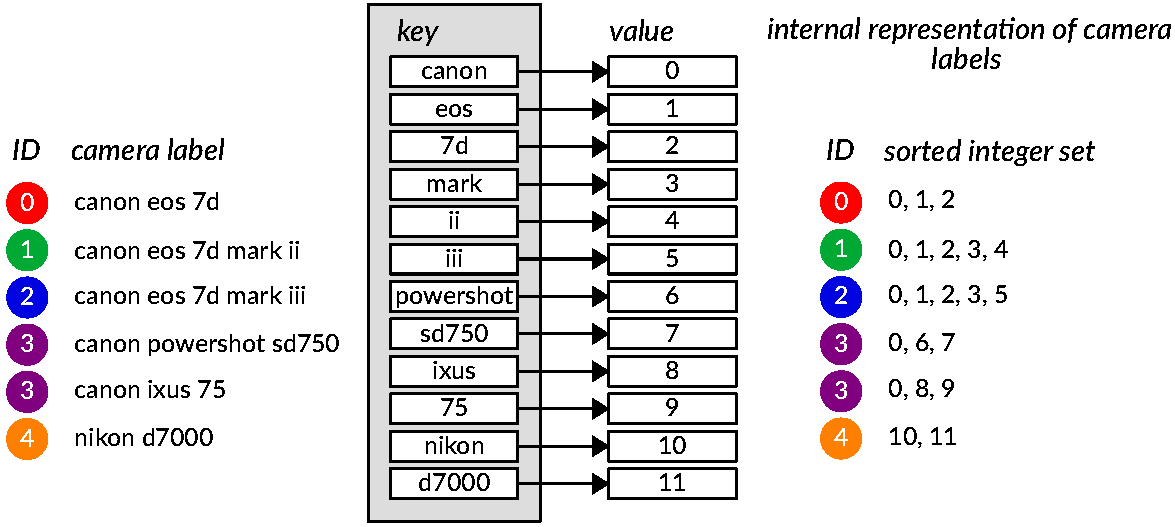
\includegraphics[width=\linewidth]{./graphics/integer_sets.pdf}
%   \caption{Conversion of mock camera labels to sorted integer sets. 
% We map each unique token (key) in camera labels to a unique value. 
% Based on these key-value-mappings, we convert camera labels to sorted integer sets. 
% A camera can have different names in different countries. Therefore, repeating IDs reference the same cameras (see, for example, ID=3).} 
%   \label{fig:integer:sets}
% \end{figure}

% \subsection{Efficient Preprocessing of Input Data}
% \label{sub:sec:preprocessing}

% The following findings are important to speed up preprocessing of the input data:

% \begin{itemize}
% \item Reading many small files concurrently, with multiple threads (compared to a single thread), takes advantage of the internal parallelism of SSDs and thus leads to higher throughput \cite{Zhuang2016}.

% \item C-string manipulation functions are often significantly faster than their C++ pendants. For example, locating substrings with \texttt{strstr} is around five times faster than using the C++ \texttt{std::string} function \texttt{find}.

% \item Hardcoding regular expressions with \emph{while, for, switch} or \emph{if-else} statements results in faster execution times than using standard RegEx libraries, where regular expressions are compiled at runtime into state machines.

% \item Changing strings in place, instead of treating them as immutable objects, eliminates allocation and copying overhead.

% \end{itemize}


% \section{Experiments}

% Table~\ref{tab:results} shows the running times of the resolution step of the five best placed teams.


% \begin{table}[htbp]
%   \caption{Comparison of the F-measure and the running times of the resolution step of the five best placed teams. The input data for the resolution step consisted of 29{,}787 in JSON formatted e-commerce websites. Measurements were taken on a
% laptop running Ubuntu 19.04 with 16 GB of RAM and two Intel Core i5-4310U CPUs. The underlying SSD was a 500\,GB 860 EVO mSATA. We cleared the page cache, dentries, and inodes before each run to avoid reading the input data from RAM instead of the SSD.}
%   \label{tab:results}
% \resizebox{\columnwidth}{!}{
%   \begin{tabular}{lcrr}
%     \toprule
%     Team& Language & F-measure & Running time (s)\\
%     \midrule
% 	PictureMe (\textbf{this paper}) &C++& 0.99 & \textbf{0.61}\\
%     DBGroup@UniMoRe &Python& 0.99 & 10.65\\
%     DBGroup@SUSTech &C++& 0.99 & 22.13\\
%     eats\_shoots\_and\_leaves &Python& 0.99 & 28.66\\
%     DBTHU &Python& 0.99& 63.21\\
%   \bottomrule
% \end{tabular}
% }
% \end{table}


\section{Conclusions}

%%
%% The next two lines define the bibliography style to be used, and
%% the bibliography file.
\bibliographystyle{ACM-Reference-Format}
\bibliography{literature}


\end{document}
\endinput
%%
%% End of file `sample-sigconf.tex'.
